% Created by Ross Barnie
% 
% Please note that I use the Java variable name convention whereby
% each consecutive word in a single variable is capitalised.
%
% This applies to all labels and references

\documentclass[a4paper]{article}

\title{User Guide: Primer Design}

\author{Ross Barnie \\
  Dmitrijs Jonins \\
  Daniel McElroy \\
  Murray Ross \\
  Ross Taylor
}
\date{}

\usepackage{url}
\usepackage{graphicx}
\graphicspath{ {../img/} }

%---------------------------------------------------------------------

\begin{document}
\maketitle
\tableofcontents
\listoffigures
\newpage

%---------------------------------------------------------------------
%---------------------------------------------------------------------

\section{About}
\label{sec:about}

This document will outline how to use the, provisionally named,
PrimerDesign application created for use by students of Molecular
Methods to learn about Polymerase Chain Reactions (PCR) and primer
design. 

If you encounter any problems while using the application, feel free
to ask your tutor, or email us at \url{TeamProjectQ@gmail.com}.

\section{Getting Started}
\label{sec:gettingStarted}

\subsection{System Requirements}
\label{sec:sysReqs}

You will need:
\begin{itemize}
\item{An operating system capable of running Java (you should not need
    to worry about this as Java runs on almost all modern Windows,
    Linux and Macintosh operating systems)}
\item{a web browser (such as Google Chrome or Mozilla
    Firefox)}
\item{Java (at least version 6) installed on your computer (most modern computers have
    Java, but if not it is freely available online from Oracle)}
\item{Access to the Molecular Methods moodle site by the School of
    Life Sciences at University of Glasgow}
\item{An internet connection (unless you have downloaded the
    application and have a DNA sequence ready)}
\end{itemize}

With that we can get started!

\subsection{Downloading and Starting the Application}
\label{sec:startingApp}

First, download the file \texttt{PrimerDesign.jar} from the Molecular
Methods moodle site and save it somewhere on your computer.
Next, double-click on the PrimerDesign.jar file you just saved,
alternatively if using a Unix-based operating system such as MacOS or
Linux you can run the application using the following terminal
command:
\begin{center}
  \verb�$ java -jar PrimerDesign.jar�
\end{center}
If you encounter problems here, ensure that you have Java installed on
your computer.

\subsection{Obtaining a DNA Sequence}
\label{sec:gettingSequence}

You will need an internet connection to perform these steps.

Now that you have successfully launched the application, you should
prepare a DNA sequence that you wish to manipulate.
As an example, we will show you how to obtain the L1CAM sequence, which
you should already be familiar with, from the NCBI (National Center
for Biotechnology Information) website at
\url{http://www.ncbi.nlm.nih.gov/}.

Use your web browser of choice to go to the NCBI website.
You should see something similar to figure \ref{fig:ncbiHome}.

\begin{figure}[hb] 
  \begin{center}
    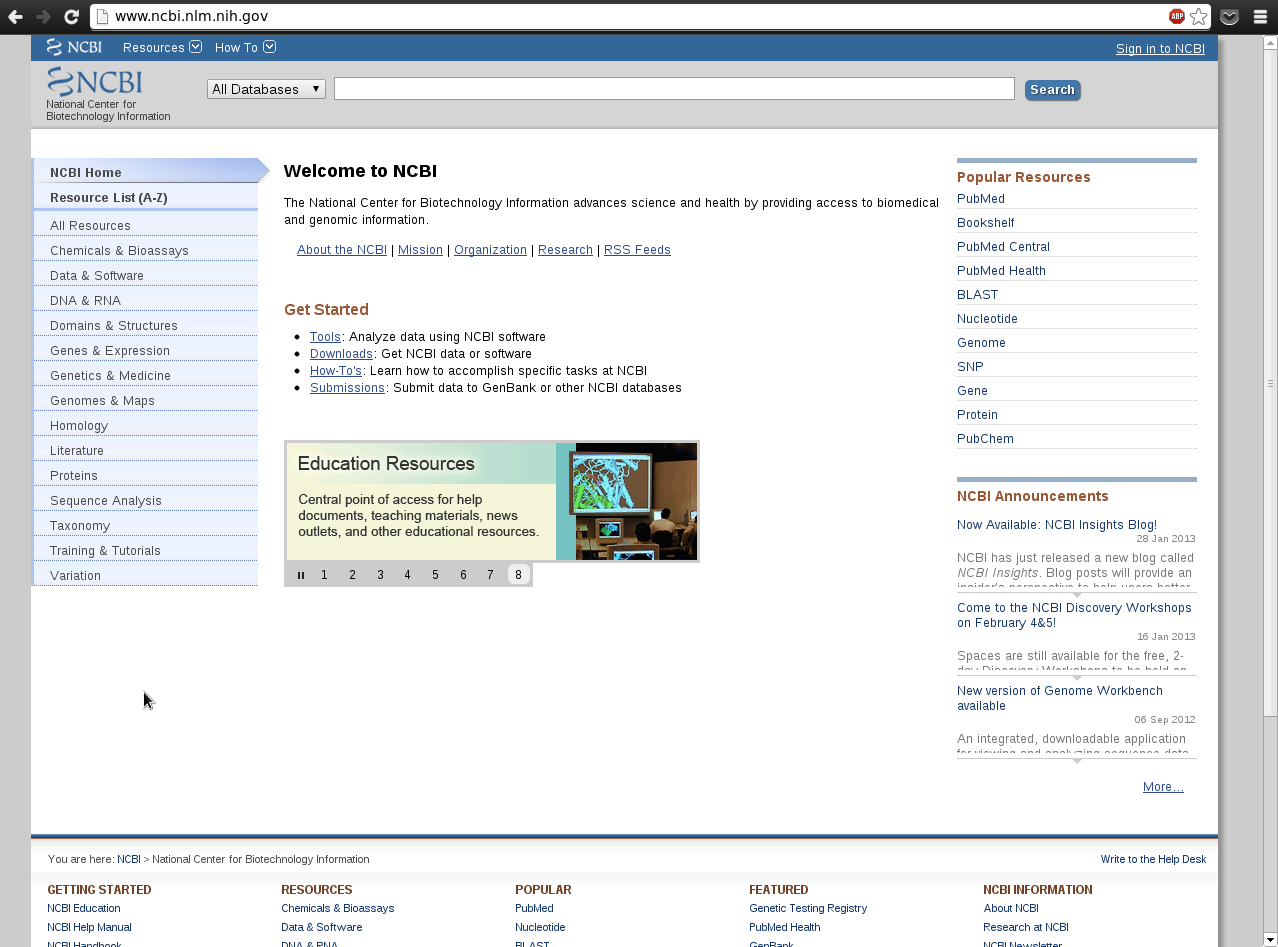
\includegraphics[width=0.8\textwidth]{ncbiHome}
    \caption{\label{fig:ncbiHome}NCBI Home Page}
  \end{center}
\end{figure}

In order to search for a compatible sequence, change the search type
to ``Nucelotides'' from the drop-down menu next to the search bar
(highlighted in yellow in figure \ref{fig:ncbiHomeSearch}) and search
for the sequence you want, for our example this is ``\verb�L1CAM�'',
using the search bar (highlighted in red in figure
\ref{fig:ncbiHomeSearch}).

\begin{figure}[hb]   
  \begin{center}
    
\includegraphics[width=\textwidth]{ncbiHomeSearch}
    \caption{\label{fig:ncbiHomeSearch}Searching for a sequence}
  \end{center}
\end{figure}

Now you will be presented with your search results, if you are
following our example click on the link highlighted in
yellow on figure \ref{fig:ncbiSearchResults}.

\begin{figure}[hb]
  \begin{center}
    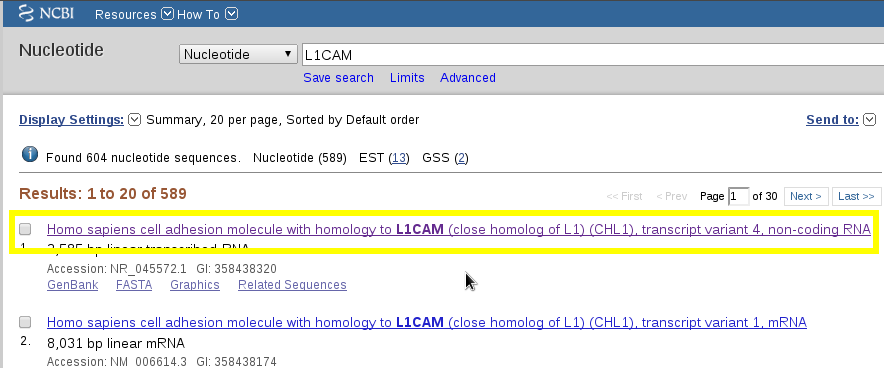
\includegraphics[width=\textwidth]{ncbiSearchResults}
    \caption{\label{fig:ncbiSearchResults}Search Results}
  \end{center}
\end{figure}

Once clicked, you should be presented with something similar to figure
\ref{fig:ncbiSequenceSelected}.

\begin{figure}[hb]
  \begin{center}
    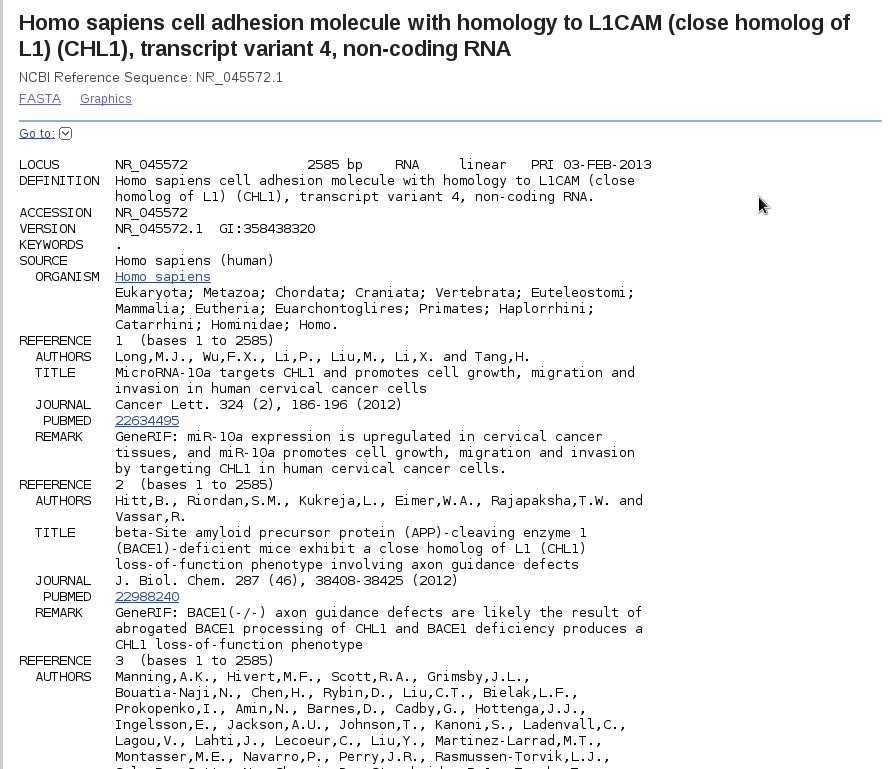
\includegraphics[width=0.8\textwidth]{ncbiSequenceSelected}
    \caption{\label{fig:ncbiSequenceSelected}Sequence Page}
  \end{center}
\end{figure}

Most of this information is irrelevant to this application, so scroll
down until you see the DNA sequence, in our example it should look
like figure \ref{fig:ncbiSequenceFound}.
Now you can simply highlight the sequence (highlighted in yellow in
figure \ref{fig:ncbiSequenceFound}) and press ctrl-c (or equivalent)
to copy the sequence.

\begin{figure}[hb]
  \begin{center}
    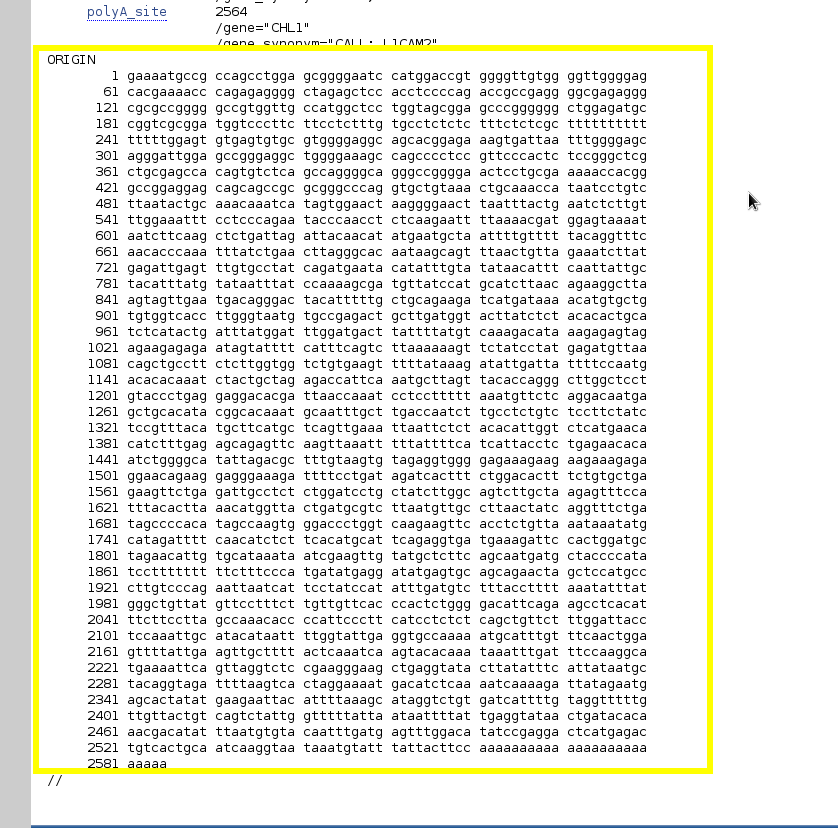
\includegraphics[width=0.8\textwidth]{ncbiSequenceFound}
    \caption{\label{fig:ncbiSequenceFound}The Sequence}
  \end{center}
\end{figure}

%--------------------------------------------------------------------
%--------------------------------------------------------------------

\section{The Application}
\label{sec:theApp}

Please note: the following information and screenshots are subject to
change and may not necessarily reflect the current build of the
system. 
Use your best judgement where differences appear.

%---------------------------------------------------------------------
\subsection{Overview Screen}
\label{sec:overviewScreen}

On starting the application (as described in section
\ref{sec:startingApp}), you should see the overview screen (figure
\ref{fig:PDSplash}) with a button on the bottom right labelled
``Start''. Once you have finished reading the information on this
page, you should press start.
Note that you will not be able to return to this page but you will be
able to view the Primer Design rules later in the application.

\begin{figure}[hb]
  \begin{center}
    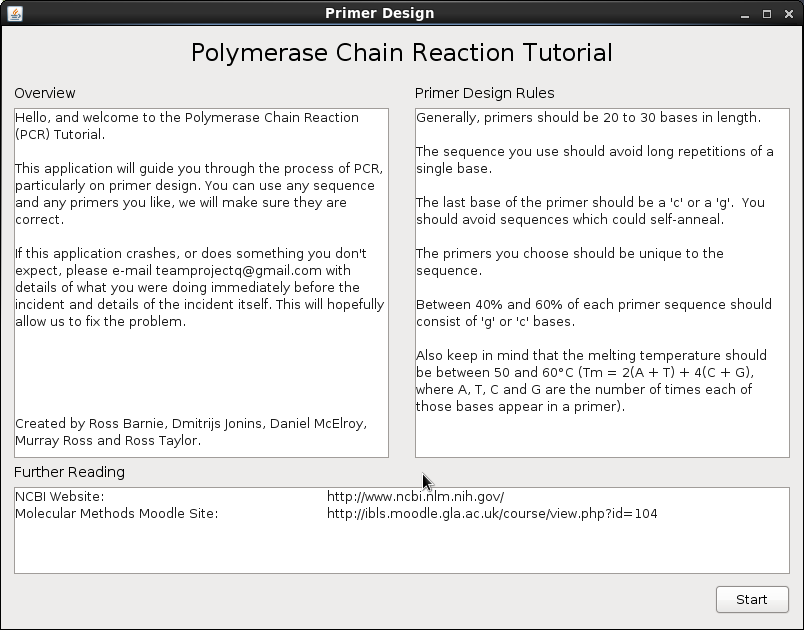
\includegraphics[width=0.8\textwidth]{PrimerDesignSplash}
    \caption{\label{fig:PDSplash}Overview Screen}
  \end{center}
\end{figure}

%---------------------------------------------------------------------

\subsection{Sequence Entry}
\label{sec:sequenceEntry}

Remember the DNA sequence you copied in section
\ref{sec:gettingSequence}? Well now is the time to paste it!
Simply paste the sequence into the large white area and press the next
button.
As you can see in figure \ref{fig:PDStartWithSeq}, you do not need to
worry about including the ``ORIGIN'' from the sequence as this will be
removed when you press the `Next' button.

\begin{figure}[hb]
  \begin{center}
    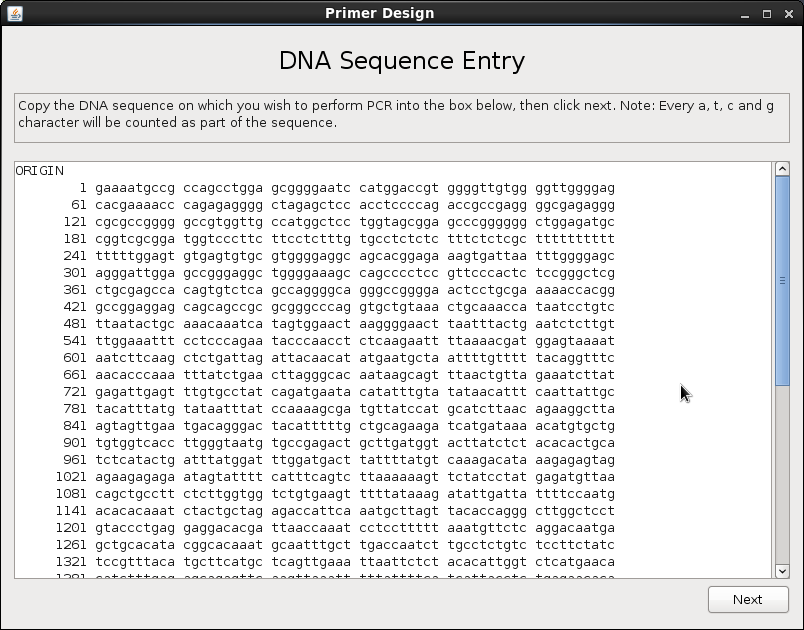
\includegraphics[width=0.8\textwidth]{PrimerDesignStartWithSeq}
    \caption{\label{fig:PDStartWithSeq}DNA Sequence Entry Example}
  \end{center}
\end{figure}

%---------------------------------------------------------------------

\subsection{Target Area Selection}
\label{sec:targetAreaSelection}

Now we have to select what it is we want to copy.
To do this, you have to specify the first and the last base of the
sequence you wish to copy, using it's position in the sequence.
So if you wish to copy a sequence from position 100 to 500, as in the
example on figure \ref{fig:PDAreaSelection}, you would enter these
into the ``From'' and ``To'' text boxes.

Note that you can also view the complementary strand, and both strands
together, by using the tabs just above where the sequence is.

\begin{figure}[hb]
  \begin{center}
    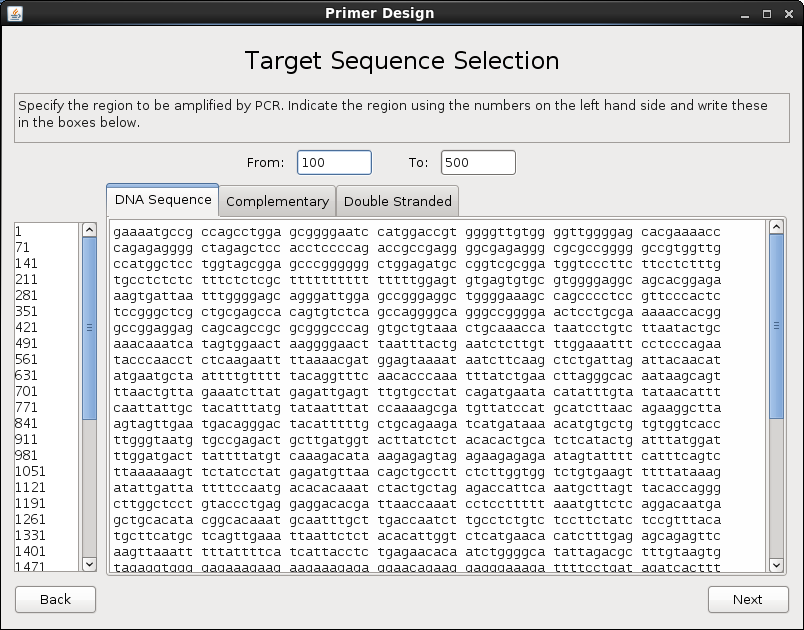
\includegraphics[width=0.8\textwidth]{PrimerDesignAreaSelection}
    \caption{\label{fig:PDAreaSelection}Target Area Selection Example}
  \end{center}
\end{figure}

%-----------------------------------
% DEMO ONLY?
Note that the sequence is split into seven blocks of 10 bases each (ie
70 bases per line).
%------------------------------------
%---------------------------------------------------------------------
\subsection{Primer Design}
\label{sec:primerDesign}

You can now see your selected area more clearly and, since primers can
include bases from before and after the target, the rest of the
sequence is still available to you.

You should design your primers and insert them into the ``Forward Primer''
and ``Reverse Primer'' fields, as shown in figure
\ref{fig:PDPrimerSelection}, note however that the example data is not
designed to be correct.

For the reverse primer, you have a button which will reverse whatever
you enter into the ``Reverse Primer'' field, the ``Reverse'' button
next the field.
So if you were to enter \verb�aattccggt�, and press the ``Reverse''
button, the primer would change to \verb�tggccttaa�.

You can also see the primer design rules again by pressing the ``Show
Primer Design Rules'' button.

\begin{figure}[hb]
  \begin{center}
    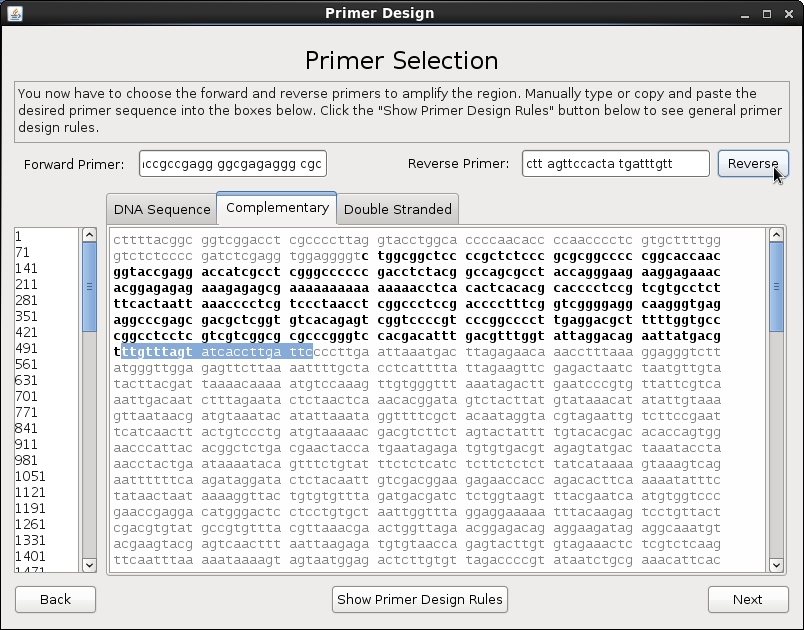
\includegraphics[width=0.8\textwidth]{PrimerDesignPrimerSelect}
    \caption{\label{fig:PDPrimerSelection}Primer Selection Example}
  \end{center}
\end{figure}

When you click next, your primers are checked against the rules
described at the start of the application, and you are given a report
of where your primers pass and where they fail, if at all.
This will look something like \ref{fig:PDPrimerFeedback}.

\begin{figure}[hb]
  \begin{center}
    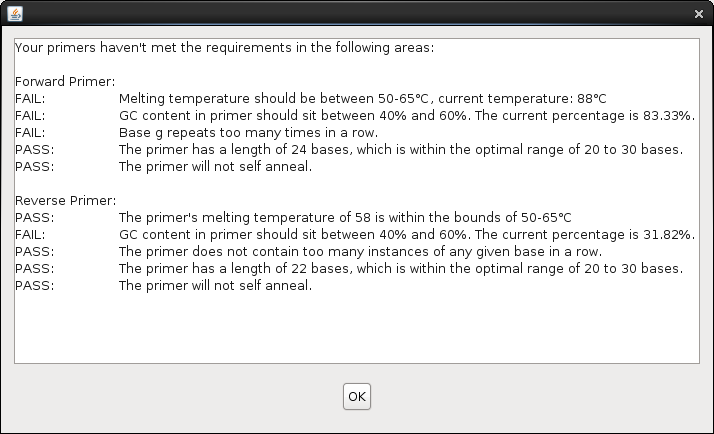
\includegraphics[width=0.8\textwidth]{PrimerDesignPrimerFeedback}
    \caption{\label{fig:PDPrimerFeedback}Primer Design Feedback Example}
  \end{center}
\end{figure}

Pressing the ``Ok'' button will close this window and allow you to
continue only if you have passed each rule.

%---------------------------------------------------------------------

\subsection{Melting Temperature}
\label{sec:meltingTemp}

Now you are finished!
This final screen, which should be similar to figure
\ref{fig:PDMeltingTemp}, lets you review your design, showing the
melting temperatures of both primers and the primers themselves.

Note that for our example we should not have been allowed to get here
due to the feedback we received in figure \ref{fig:PDPrimerFeedback}.

\begin{figure}[hb]
  \begin{center}
    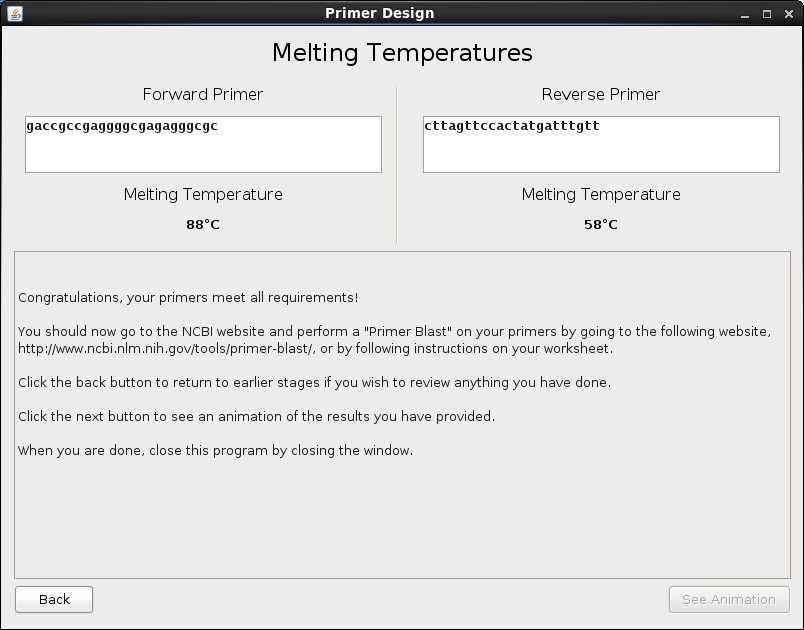
\includegraphics[width=0.8\textwidth]{PrimerDesignMeltingTemp}
    \caption{\label{fig:PDMeltingTemp}Melting Temperature Screen Example}
  \end{center}
\end{figure}

\subsubsection{\date{8th February 2013} Demonstration Only}
Also please note that although we have included the ``See Animation''
button, it is currently not working so we have disabled it.

\end{document}